%%%%%%%%%%%%%%%%%%%%%%%%%%%%%%%%%%%%%%%
% PlushCV - One Page Two Column Resume
% LaTeX Template
% Version 1.0 (11/28/2021)
%
% Author:
% Shubham Mazumder (http://mazumder.me)
%
% Hacked together from:
% https://github.com/deedydas/Deedy-Resume
%
% IMPORTANT: THIS TEMPLATE NEEDS TO BE COMPILED WITH XeLaTeX
%
%%%%%%%%%%%%%%%%%%%%%%%%%%%%%%%%%%%%%%

\documentclass[]{plushcv}
\usepackage{fancyhdr}
\usepackage{tikz} % Hinzugefügt für das Profilbild
\pagestyle{fancy}
\fancyhf{}

\begin{document}
	
	% =========================================================
	% HAUPTFARBE HIER ÄNDERN (Muss zwingend nach \begin{document} stehen!)
		% =========================================================
		\definecolor{primary}{RGB}{242, 142, 7}  %Firmenfarbe
		% --- DER NEUE FIX FÜR DEN FEHLER ---
		\colorlet{PRIMARY}{primary} % Fängt ab, wenn das Template den Text großschreibt!
		% -----------------------------------
		
		% Diese Befehle zwingen die Vorlagen-Variablen auf deine Farbe:
		\colorlet{headings}{gray}
		\colorlet{subheadings}{black}
		% =========================================================
		
		% --- PORTRAIT FOTO ---
		\begin{tikzpicture}[remember picture,overlay]
			\node[anchor=north east, inner sep=0pt, xshift=-0.5cm, yshift=-0.5cm] at (current page.north east) {
				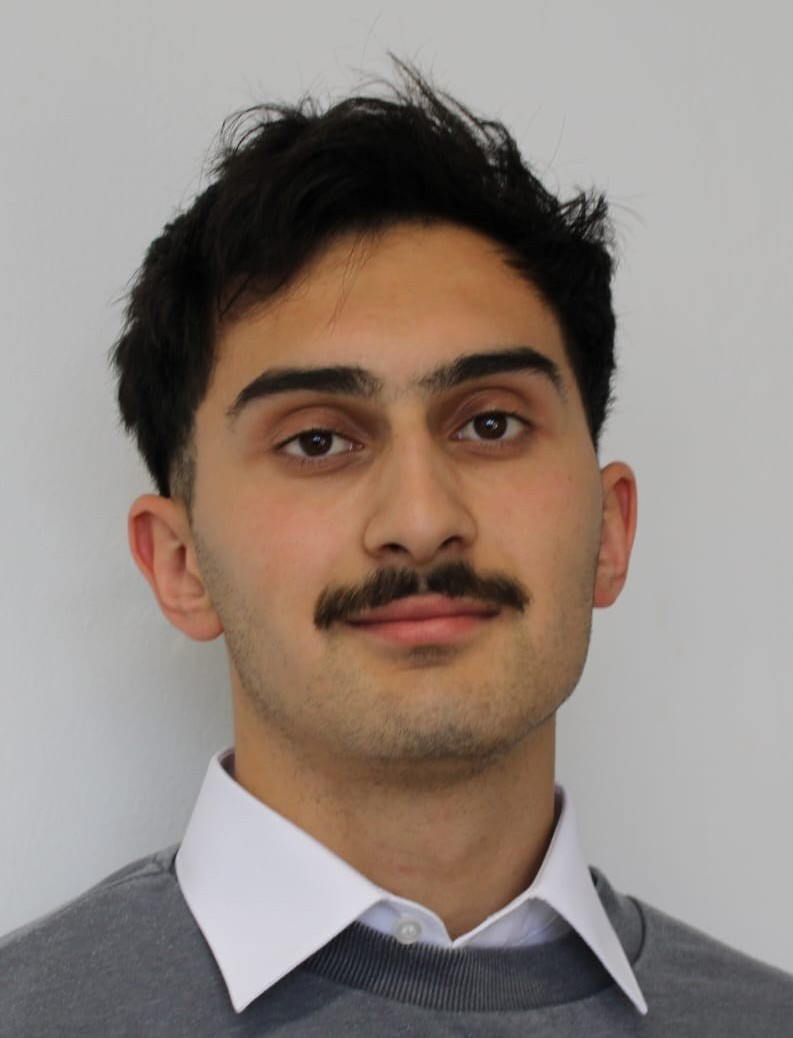
\includegraphics[height=4.5cm]{foto.jpeg} % <-- Hier deinen Dateinamen eintragen
			};
		\end{tikzpicture}
		% ---------------------
		
		%%%%%%%%%%%%%%%%%%%%%%%%%%%%%%%%%%%%%%
		%     TITLE NAME
		%%%%%%%%%%%%%%%%%%%%%%%%%%%%%%%%%%%%%%
		
		\namesection{\color{primary}Felix}{\color{primary}Raffl}{\color{primary}Master Mechatronics Student}{
			
\includegraphics[scale=0.30,trim={0 1cm 0cm 0cm}]{icons/main/linkedin.png}\hspace{0.1cm}\href{https://www.linkedin.com/in/felix-raffl-277116266}{Felix Raffl} \hspace{0.5cm} 
			
\includegraphics[scale=0.30,trim={0 1cm 0cm 0cm}]{icons/main/mail.png}\hspace{0.1cm}\href{mailto:felix.raffl7@gmail.com}{felix.raffl7@gmail.com} \hspace{0.5cm} 
			
\includegraphics[scale=0.30,trim={0 1.25cm -0.4cm 0cm}]{icons/main/phone.png}\hspace{0.1cm}\href{tel:+393894442477}{+393894442477}
		}
		
		%%%%%%%%%%%%%%%%%%%%%%%%%%%%%%%%%%%%%%
		%     OBERER BEREICH: 70% / 25% SPLIT
		%%%%%%%%%%%%%%%%%%%%%%%%%%%%%%%%%%%%%%
		
		\begin{minipage}[t]{0.70\textwidth} 
			
			\section{\color{primary}Arbeitserfahrung und Praktika}
			
			\runsubsection{}%
			\href{https://research.mci.edu/de/pra}{\runsubsection{\color{primary}Zentrum für Produktion, Robotik \& Automatisierung}}
			\descript{| Bachelorand}
			\location{März 2025 – August 2025 | Innsbruck, Österreich}
			\vspace{\topsep}
			\begin{tightemize}
				\sectionsep
				\item Bachelorarbeit im Bereich der Laborautomatisierung.
				\item Entwicklung eines Robotersystems zur Automatisierung von Prozessen in der Hämatologie.
				\item Entwicklung einer Schulungsplattform für die Vorlesung  "Robotic Systems in Sports and Medical Technology" für den Bachelorstudiengang Medizin-, Gesundheits- \& Sporttechnologie am MCI.
			\end{tightemize}
			\sectionsep
			
			\runsubsection{}%
			\href{https://www.zfx-dental.com/}{\runsubsection{\color{primary}Zfx Dental}}
			\descript{Praktikum im Bereich Qualitätskontrolle und Konstruktion}
			\location{Juli 2024 – September 2024 | Gargazon, Italien}
			\begin{tightemize}
				\sectionsep
				\item Programmierung von Messabläufen für Bruker alicona µCMM
				\item Kontrolle und Bearbeitung von Reklammationsartikeln
				\item Kontruktion von Scankörpern zur Platzierung von Zahnimplanaten
			\end{tightemize}
			\sectionsep
			
			\runsubsection{}%
			\href{https://www.drschaer.com/de/}{\runsubsection{\color{primary}Dr. Schär}}
			\descript{Praktikum im Bereich Technik}
			\location{Juli 2023 – September 2023 | Burgstall, Italien}
			\begin{tightemize}
				\sectionsep
				\item Wartungsarbeiten an der Produktionslinie
				\item Inventar des Ersatzteillagers
			\end{tightemize}
			\sectionsep
			
			\runsubsection{}%
			\href{https://www.iprona.com/}{\runsubsection{\color{primary}iprona Group}}
			\descript{Praktikum im Bereich Technik}
			\location{Mai 2021 – September 2021 | Lana, Italien}
			\begin{tightemize}
				\sectionsep
				\item Zeichnung von Elektroschaltplänen
				\item Wartungsarbeiten an der Produktionslinie
			\end{tightemize}
			\sectionsep
			
		\end{minipage} 
		\hfill
		\begin{minipage}[t]{0.25\textwidth} 
			
			\section{\color{primary}Kenntnisse}
			\subsection{\color{primary}Programmierung}
			\sectionsep
			\textbullet{}Robotstudio/Rapid \\\textbullet{}Python\\ \textbullet{}C++ \\\textbullet{}\LaTeX \\ \textbullet{}Beckhoff TwinCAT\\
			\textbullet{}CodeSys
			\sectionsep
			
			\subsection{\color{primary}Konstruktion}
			\sectionsep
			\textbullet{}Inventor \\ \textbullet{}AutoCAD \\ \textbullet{}Eagle \\ \textbullet{}SolidWorks \\
			\sectionsep
			
		\end{minipage} 
		
		\vspace{0.5cm} % Etwas Abstand zwischen dem oberen und unteren Bereich
		
		%%%%%%%%%%%%%%%%%%%%%%%%%%%%%%%%%%%%%%
		%     UNTERER BEREICH: 50% / 50% SPLIT (Volle Breite)
		%%%%%%%%%%%%%%%%%%%%%%%%%%%%%%%%%%%%%%
		
		\begin{minipage}[t]{0.48\textwidth}
			\section{\color{primary}Ausbildung} 
			
			\runsubsection{}%
			\href{https://www.mci.edu/de/studium/master/mechatronics-smart-technologies}{\runsubsection{\color{primary}Master am MCI}}
			\descript{Master in Mechatronik – Smart Technologies}
			\location{Okt. 2025 - Aktuell | Innsbruck, AT}
			\location{Aktueller Notendurchschnitt: 2.12}
			
			\sectionsep
			
			\runsubsection{}%
			\href{https://www.mci.edu/de/studium/bachelor/medizin-gesundheits-und-sporttechnologie}{\runsubsection{\color{primary}Bachelor am MCI}}
			\descript{Bachelor in Medizin-, Gesundheits- \& Sporttechnologie}
			Bachelorarbeit: Anpassung und Erweiterung einer
			Lernplattform für robotische Systeme in
			der Laborautomatisierung\newline
			\location{Okt. 2022 - Sept. 2025 | Innsbruck, AT}
			\location{Mit ausgezeichnetem Erfolg bestanden}
			\sectionsep
			
			\runsubsection{}%
			\href{https://www.tfo-meran.it/}{\runsubsection{\color{primary}Technologische Fachoberschule Meran}}
			\descript{Matura in Elektronik \& Elektrotechnik}
			Maturaarbeit: Füllstandsmessung der Trinkwasserreservoire Kuens\newline
			\location{Sept. 2017 - Juli 2022 | Meran, IT}
			\location{Mit 87 von 100 Punkte bestanden}
		\end{minipage}
		\hfill
		\begin{minipage}[t]{0.48\textwidth}
			\section{\color{primary}Projekte}
			
			\runsubsection{\color{primary}Inbetriebnahme eines robotischen Systems zur Qualitätskontrolle mit Conveyor-Tracking}
			\descript{| Robotstudio/Rapid, Cognex In-Sight-Vision}
			\location{2026}
			\vspace{0.5cm} % Puffer für den Zeilenumbruch im Titel
			\begin{tightemize}
				\item Cognex-Kamerajob zur Qualitätskontrolle
				\item Roboterprogrammierung mit Conveyor-Tracking
			\end{tightemize}
			\sectionsep
			
			\runsubsection{\color{primary}Konzept und Prototyp eines Systems zur Erfassung von Wiederholungen im Krafttraining}
			\descript{| C++}
			\location{2024}
			\vspace{0.1cm} % Angepasster Abstand für symmetrische Optik
			\begin{tightemize}
				\item Entwicklung der elektronischen Schaltung
				\item Entwicklung der Software zum Auswerten des Beschleunigungssensors
			\end{tightemize}
			\sectionsep
		\end{minipage}
		
	\end{document}